\documentclass[../main.tex]{subfiles}
\begin{document}
\chapter{Channel Coding}
This chapter discusses communication through a noisy channel reliably at optimal rate.
\section*{Discrete Memoryless Channel DMC}
Binary Symmetric Channel (BSC): the simplest possible channel.
\begin{itemize}
    \item input alphabet $\X=\{0,1\}$
    \item output alphabet $\Y=\{0,1\}$
    \item crossover probability $=\epsilon$, $0\leq\epsilon\leq 1$.
    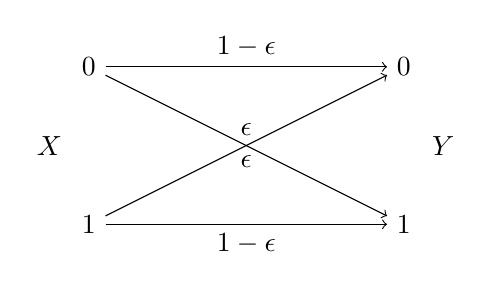
\begin{tikzpicture}
    % Nodes
    \node at (0, 2) (X0) {0};
    \node at (0, 0) (X1) {1};
    \node at (4, 2) (Y0) {0};
    \node at (4, 0) (Y1) {1};
    \node at (-0.5, 1) (X) {$X$};
    \node at (4.5, 1) (Y) {$Y$};
    
    % Arrows and labels
    \draw[->] (X0) -- (Y0) node[midway, above] {$1-\epsilon$};
    \draw[->] (X0) -- (Y1) node[midway, below] {$\epsilon$};
    \draw[->] (X1) -- (Y0) node[midway, above] {$\epsilon$};
    \draw[->] (X1) -- (Y1) node[midway, below] {$1-\epsilon$};
\end{tikzpicture}
\end{itemize}
A simple code:
\begin{itemize}
    \item Assume $\epsilon < 0.5$.
    \item Two possible messages $A,B$ are to be sent throug the channel. 
    \item Coding scheme 1: \[
    Encoding \begin{cases}
        A\to 0\\
        B\to 1
    \end{cases}
    \]
    \[Decoding \begin{cases}
    0\to A\\
    1\to B
        \end{cases}\]
    \item a decoding error occurs if and only if a crossover occurs. Therefore $P_e=\epsilon$
\end{itemize}
A more elaborated code: repetition code:
\begin{itemize}
    \item To improve reliability, use the BSC $n$ ties for a large $n$.
    \item Let $N_0=\#0$'s received and $N_1=\#1$'s received.
    \item Coding scheme 2: \[
    Encoding \begin{cases}
        A \to 00\dots 0\\
        B \to 11\dots 1
    \end{cases}
    Decoding \begin{cases}
        N_0 > N_1 \to A\\
        N_0 > N_1 \to B
    \end{cases}
    \] 
    \item If the message if $A$, by WLLN, $N_0\to n(1-\epsilon)$ and $N_1\to n\epsilon$ in probability.
    \item The decoding rate goes to $1$.
    \item However, coding rate $R=\frac{1}{n}\log 2\to 0$ as $n\to \infty$. Coding rate is the amount of information transmitted per use of the channel.
\end{itemize}
\section{7.1 Definition and Capacity}
 \begin{pbox}{Discrete Memoryless Channel 1}
     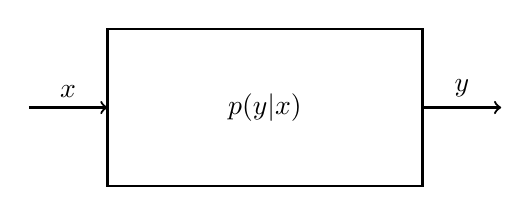
\begin{tikzpicture}[thick]
    % Draw the box
    \draw (0,0) rectangle (4,2);
    
    % Input arrow
    \draw[->] (-1,1) -- (0,1) node[midway, above] {$x$};
    
    % Output arrow
    \draw[->] (4,1) -- (5,1) node[midway, above] {$y$};
    
    % Label inside the box
    \node at (2,1) {$p(y|x)$};
\end{tikzpicture}
\begin{itemize}
    \item Single input random variable $X$ takes values in discrete alphabet $\X$.
    \item Single Output random variable takes values in discrete output alphabet $\Y$.
    \item The channel is specified by a transition matrix $p(y|x)$ from $\X$ to $\Y$.
    \item Input-output relation: \[
    Pr\{X=x, Y=y\}=Pr\{X=x\} p(y|x)
    \]
    \item BSC with cross probability $\epsilon$ \[
    [p(y|x)]=\begin{bmatrix}
        1-\epsilon & \epsilon\\
        \epsilon & 1- \epsilon
    \end{bmatrix}
    \]
\end{itemize}
 \end{pbox}
 \begin{pbox}{Discrete Memoryless Channel 2}
     \begin{tikzpicture}[thick]
    % Nodes
    \node at (-2, 0) (X) {$X$};
    \node at (0, 0) (circle) [draw, circle] {$\alpha$};
    \node at (2, 0) (Y) {$Y$};
    \node at (0, 2) (Z) {$Z$};
    
    % Arrows
    \draw[->] (X) -- (circle);
    \draw[->] (circle) -- (Y);
    \draw[->] (Z) -- (circle);
    
    % Labels
    \node at (0, -0.5) {};
\end{tikzpicture}
\begin{itemize}
    \item Input random variable $X$ takes values in discrete alphabet $\X$.
    \item Output random variable takes values in discrete output alphabet $\Y$.
    \item Noise variable $Z$ takes values in discrete alphabet $\Z$
    \item $Z$ is independent of $X$
    \item $\alpha$ is a function from $\X\times \Z$ to $\Y$  
    \item Input-output relation: \[
    Y=\alpha(X,Z)
    \]
    \item The channel is specified by $(\alpha, Z)$
    \item The channel is specified by a transition matrix $p(y|x)$ from $\X$ to $\Y$.
    \item Input-output relation: \[
    Pr\{X=x, Y=y\}=Pr\{X=x\} p(y|x)
    \] 
\end{itemize}
\end{pbox}
Equivalence of Discrete Channel 1 and Discrete Channel 2.
\newline
If a channel can be modeled by DS2, then it can also be modeled by discrete channel 1. Given we can let $p(y|x)=Pr(a(X,Z)=y|X=x) = P(\alpha(x,Z)=y)$, by independence.
\newline
If a channel can be modeled by DS1, then it can also be modeled by discrete channel 2.\\
For $x\in \X$, define $Z_x$ with $\Z_x=\Y$ such that $Pe\{Z_x=y\}=p(y|x)$.\\
Assume that $Z_x,x\in\X$ are mutually independent and also independent of $X$.\\
Define the noise $Z=(Z_x:x\in\X)$.
Let $Y=Z_x$ if $X=x$ so that $Y=\alpha(X,Z)$.
\newline
\begin{align*}
\Pr\{X = x, Y = y\} &= \Pr\{X = x\}\Pr\{Y = y \mid X = x\} \\
&= \Pr\{X = x\}\Pr\{Z_x = y \mid X = x\} \\
&= \Pr\{X = x\}\Pr\{Z_x = y\}\\
&= Pr\{X=x\}p(y|x)
\end{align*}
\begin{pbox}{Equivalence of channels}
    2 channels $p(y|x)$ and $(\alpha,Z)$ are equivalent if \[
    Pr\{\alpha(x,Z)=y\} = p(y|x)
    \] for all $x$ and $y$.
\end{pbox}

\section{Discrete Memoryless Channel}
\begin{itemize}
    \item A discrete channel can be used repeatedly at every time index $i=1,2,\dots$.
    \item Assume the noise for th transmission over the channel at different time indices are independent of each other.
    \item We regard DMC as a subsystem of a discrete-time stochastic system which will be referred to as "the system".
    \item In such a system, random variables are generated sequentially in discrete-time.
    \item More than one random variable may be generated instantaneously, but sequentially at a particular time index.
\end{itemize}

\begin{pbox}{DMC 1}
\begin{center}
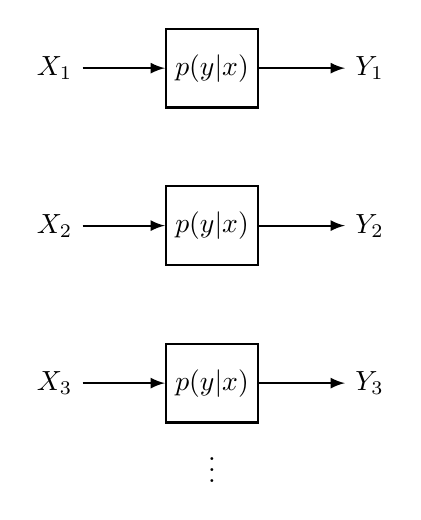
\begin{tikzpicture}[thick, >=latex]

    % Nodes
    \node at (-2, 2) (X1) {$X_1$};
    \node at (0, 2) (C1) [draw, rectangle, minimum width=1cm, minimum height=1cm] {$p(y|x)$};
    \node at (2, 2) (Y1) {$Y_1$};
    
    \node at (-2, 0) (X2) {$X_2$};
    \node at (0, 0) (C2) [draw, rectangle, minimum width=1cm, minimum height=1cm] {$p(y|x)$};
    \node at (2, 0) (Y2) {$Y_2$};
    
    \node at (-2, -2) (X3) {$X_3$};
    \node at (0, -2) (C3) [draw, rectangle, minimum width=1cm, minimum height=1cm] {$p(y|x)$};
    \node at (2, -2) (Y3) {$Y_3$};
    
    % Arrows
    \draw[->] (X1) -- (C1);
    \draw[->] (C1) -- (Y1);
    
    \draw[->] (X2) -- (C2);
    \draw[->] (C2) -- (Y2);
    
    \draw[->] (X3) -- (C3);
    \draw[->] (C3) -- (Y3);
    
    % Dots
    \node at (0, -3) {$\vdots$};
    
\end{tikzpicture}
\end{center}
\begin{itemize}

    \item A DMC specified by $p(y|x)$ is a sequence of replicates of a generic discrete channel $p(y|x)$
    \item Let $T_{i-}$ be the collection of all random variables in the system generated before $X_i$.
    \item Memoryless property (independent noise): \[
    Pr\{Y_i=y, X_i=x,T_{i-}=t\}\\
    =Pr\{X_i=x, T_{i-}=t\}p(y|x)
    \]
    \item note that $p(y|x)$ represents $Pr(Y_i=y|X_i=x|T_{i-}=t)$
    \item Equivalently, $T_{i-}\to X_i\to Y_i$ forms a Markov chain.
\end{itemize}
\end{pbox}


\begin{pbox}{DMC 2 alternative definition}
    \begin{center}
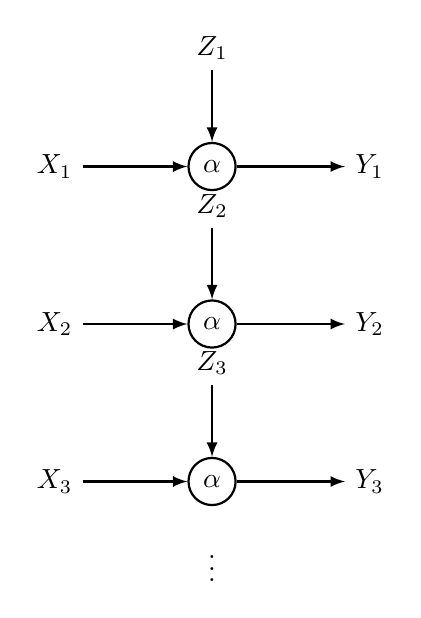
\begin{tikzpicture}[thick, >=latex]

    % Nodes for the first row
    \node at (-2, 2) (X1) {$X_1$};
    \node at (0, 2) (circle1) [draw, circle] {$\alpha$};
    \node at (2, 2) (Y1) {$Y_1$};
    \node at (0, 3.5) (Z1) {$Z_1$};
    
    % Nodes for the second row
    \node at (-2, 0) (X2) {$X_2$};
    \node at (0, 0) (circle2) [draw, circle] {$\alpha$};
    \node at (2, 0) (Y2) {$Y_2$};
    \node at (0, 1.5) (Z2) {$Z_2$};
    
    % Nodes for the third row
    \node at (-2, -2) (X3) {$X_3$};
    \node at (0, -2) (circle3) [draw, circle] {$\alpha$};
    \node at (2, -2) (Y3) {$Y_3$};
    \node at (0, -0.5) (Z3) {$Z_3$};
    
    % Dots for continuation
    \node at (0, -3) {$\vdots$};
    
    % Arrows for the first row
    \draw[->] (X1) -- (circle1);
    \draw[->] (circle1) -- (Y1);
    \draw[->] (Z1) -- (circle1);
    
    % Arrows for the second row
    \draw[->] (X2) -- (circle2);
    \draw[->] (circle2) -- (Y2);
    \draw[->] (Z2) -- (circle2);
    
    % Arrows for the third row
    \draw[->] (X3) -- (circle3);
    \draw[->] (circle3) -- (Y3);
    \draw[->] (Z3) -- (circle3);
    
\end{tikzpicture}
\end{center}
\begin{itemize}
    \item A DMC specified by $(\alpha, Z)$ is a sequence of replicates of a generic discrete channel $(\alpha, Z)$. The output of the DMC at time $i$ is given by $Y_i=\alpha(X_i,Z_i)$
    \item $Z_i$ is the noise variable for transmission at time $i$, and has the same distribution as $Z$.
    \item Memoryless Property (Independent noise): $Z_i$ is independent of $(X_i, T_{i-})$
    \item This channel is equivalent to the DMC 1 above.
\end{itemize}
\end{pbox}
\begin{gbox}{Capacity of a channel}
    The capacity of a discrete memoryless channel $p(y|x)$ is defined as \[
    C =\max_{p(x)}I(X;Y), 
    \] where $X$ and $Y$ are respectively the input and th output of the generic discrete channel, and the maximum is taken over all input distributions $p(x)$.
\end{gbox}
For each input didtribution $p(x)$, we have \[
p(x,y)=p(x)p(y|x)
\]
From $p(x,y)$, we can compute $I(X;Y)$. Maximize $I(X;Y)$ over all input distributions.
\begin{remark}
    Since $I(X;Y)$ is a continuous functional of $p(x)$ and the set of all $p(x)$ is a compact set, closed and bounded in $\mathcal{R}^{|\X|}$, the maximum value of $I(X;Y)$ can always be attained.
    \newline
    We will see that $C$ is the maximum rate at which information can be reliably communicate through a DMC.
    \newline
    We will see that we can communicate through a channel with positive rate while $P_e\to 0$.
\end{remark}
\begin{pbox}{Example BSC}
    Consider $Y=X+Z\mod 2$, with \[
    P(Z=0)=1-\epsilon, P(Z=1)=\epsilon
    \] and $Z$ is independent of $X$. (If $Z=1$, crossover occurs.)\\
    \begin{align*}
        I(X;Y)&=H(Y)-H(Y|X)\\
        &= H(Y)-\sum_xp(x)H(Y|X=x)\\
        &=H(Y)-\sum_xp(x)h_b(\epsilon)\\
        &=H(Y)-h_b(\epsilon)\\
        &\leq 1-h_b(\epsilon) \quad \text{because $Y$ carries at most 1 bit of information}
    \end{align*}
    Therefore \begin{align*}
        C=\max_{p(x)}I(X;Y)
        \leq 1-h_b(\epsilon)
    \end{align*}
    The upper bound on $I(X;Y)$ is tight if $H(Y=1)$, and this can be achieved by taking the uniform input distribution.
    \newline 
    We say that the channel has capacity $C=1-h_b(\epsilon)$ bit per use.
    \begin{remark}
    \begin{itemize}
        \item when $\epsilon=0$, $C(0)=1$. Intuitively, this means the channel doesn't error and we can communicate information at 1 bit per use.
        \item When $\epsilon=1$, $C(0)=1$ as well. This is symmetric to the case $\epsilon=0$ where the decoder just flips the information.
        \item $X$ and $Y$ are independent for $\epsilon=0.5$, in this case, we cannot communicate information. Also $Y$ follows unfirom distribution in this case.
    \end{itemize}
\end{remark}
\end{pbox}
\begin{pbox}{Example: Binary Erasure Channel}
\begin{center}
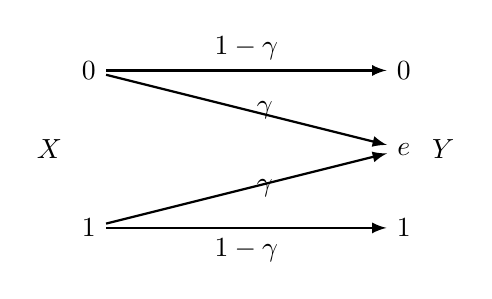
\begin{tikzpicture}[thick, >=latex]

    % Nodes
    \node at (-2, 2) (X0) {0};
    \node at (-2, 0) (X1) {1};
    \node at (2, 2) (Y0) {0};
    \node at (2, 0) (Y1) {1};
    \node at (2, 1) (Ye) {$e$};
    \node at (-2.5, 1) (X) {$X$};
    \node at (2.5, 1) (Y) {$Y$};
    
    % Arrows and labels
    \draw[->] (X0) -- (Y0) node[midway, above] {$1-\gamma$};
    \draw[->] (X0) -- (Ye) node[midway, right] {$\gamma$};
    \draw[->] (X1) -- (Ye) node[midway, right] {$\gamma$};
    \draw[->] (X1) -- (Y1) node[midway, below] {$1-\gamma$};
    
\end{tikzpicture}
\end{center}
    \begin{itemize}
        \item The output symbol $e$ denotes "erasure."
        \item $\gamma$: Erasure probability $0\leq \gamma \leq 1$.
        \item With probability $1-\gamma$, $Y=X$ (regardless of whether $X=0$ or $X=1$)
        \item With probability $\gamma,$ $Y=e$ (erasure)
        \item Note there is either no error, or there is an erasure. 
    \end{itemize}
    \begin{align*}
        C&=\max_p(x) I(X;Y)\\
        &=\max_{p(x)}H(Y)-H(Y|X)\\
        &=\max_{p(x)}H(Y)-h_b(\gamma)\\
        &= (1-\gamma)\max_{p(0)}h_b(p(0))
    \end{align*}
    The channel capacity is $1-\gamma$ per use.
\end{pbox}

\section{The Channel Coding Theorem}
\begin{itemize}
    \item Direct direction: Information can be communicated through a DMC with an arbitrarily small probability of error at any rate less than the channel capacity.
    \item Converse: If information is communicated through a DMC at a rate higher than the capacity, then the probability of error is bounded away from zero.
\end{itemize}
\begin{gbox}{Channel Code}
    An $(n,M)$ code for a discrete memoryless channel with input alphabet $\X$ and output alphabet $\Y$ is defined by an encoding function\[
    f:\{1,\dots,M\}\to \X^n
    \] 
    and a decoding function
    \[
    g:\Y^n \to \{1,2,\dots,M\}.
    \]
\begin{itemize}
    \item n: block length
    \item $\mathcal{W}=\{1,\dots,M\}$: Message Set
    \item $f(1),\dots,f(M)$: codewords
    \item the set of all codewords: codebook
\end{itemize}
\end{gbox}
Assumptions:
\begin{itemize}
    \item $W$ is uniformly chosen from the message set $\mathcal{W}$, so $H(W)=\log M$
    \item $\vec X=(X_1,...,X_n), \vec Y=(Y_1,\dots,Y_n)$.
    \item Thus $X=f(W)$, i.e. the transmitted sequence is a codeword for the chosen message.
    \item Let $\hat{W}=g(\vec Y)$ denote the estimate on the message $W$ by the decoder.
\end{itemize}
\begin{center}
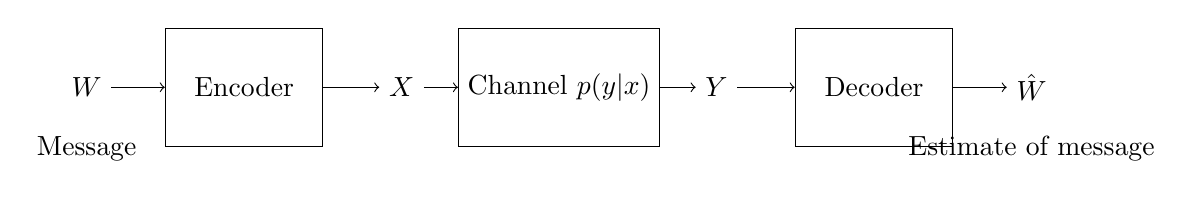
\begin{tikzpicture}

    % Nodes
    \node at (-4, 0) (W) {$W$};
    \node at (-4, -0.5) [below] {Message};
    \node at (-2, 0) (encoder) [draw, rectangle, minimum width=2cm, minimum height=1.5cm] {Encoder};
    \node at (0, 0) (X) {$X$};
    \node at (2, 0) (channel) [draw, rectangle, minimum width=2cm, minimum height=1.5cm] {Channel $p(y|x)$};
    \node at (4, 0) (Y) {$Y$};
    \node at (6, 0) (decoder) [draw, rectangle, minimum width=2cm, minimum height=1.5cm] {Decoder};
    \node at (8, 0) (W_hat) {$\hat{W}$};
    \node at (8, -0.5) [below] {Estimate of message};
    
    % Arrows
    \draw[->] (W) -- (encoder);
    \draw[->] (encoder) -- (X);
    \draw[->] (X) -- (channel);
    \draw[->] (channel) -- (Y);
    \draw[->] (Y) -- (decoder);
    \draw[->] (decoder) -- (W_hat);
    
\end{tikzpicture}
\end{center}
Performance Measures of the channel code
\begin{gbox}{Error Probability}
    For all $1\leq w\leq M$, let \[
    \lambda_w=Pr\{\hat{W}\neq w|W=w\}=\sum_{\vec y\in Y^n:g(\vec y)\neq w}Pr\{\vec Y=\vec y|\vec X=f(w)\}
    \]
    be the conditional probability of error given the message is $w$.
\newline
The maximal probability of error of an $(n,M)$ code is $\lambda_{max}=\max_w\lambda_w$. It's the error probability of the worst codeword.
\newline
The average probability of error of an $(n,M)$ code is defined as \[
P_e=Pr\{\hat{W}\neq W\}
\]
\end{gbox}
$P_e$ and $\lambda_{max}$
Consider \begin{align*}
    P_e &= \Pr\{\hat{W}\neq W\}\\
    &=\sum_w \Pr(W=w) \Pr(\hat{W}\neq W|W=w)\\
    &= \sum_w \frac{1}{M}\Pr(\hat{W}\neq w|W=w)\\
    &=\frac{1}{M}\sum_w \lambda_w
\end{align*}
So \[
P_e\leq \max_w \lambda_w\leq \lambda_{max}
\]
\begin{gbox}{Rate of a Channel Code}
   The rate of an $(n,M)$ channel code is $n^{-1}\log M$ in bits per use.
   \newline
   A rate $R$ is asymptotically \textbf{achievable} for a discrete memoryless channel if for any $\epsilon>0$, for sufficiently large $n$ there exists an $(n,M)$ code such that \[
   \frac{1}{n}\log M>R-\epsilon
   \]
   and \[
   \lambda_{max}<\epsilon
   \]
   \end{gbox}
   The following is our main theorem of the chapter.
   \begin{bbox}{Channel Coding Theorem}
       A rate $R$ is achievable for a discrete memoryless channel if and only if $R\leq C$, the capacity of the channel.
   \end{bbox}

Now we prove the converse of the channel coding theorem.
\begin{itemize}
    \item The communication system consists of the r.v.'s $W,X_1,Y_1,\dots,X_n,Y_n,\hat{W}$.
    \item The memorylessness of the DMC imposes the following Markov constraint for each $i:$\[
    (W,X_1,Y_1,\dots, X_{i-1},Y_{i-1})\to X_i\to Y_i
    \]
    \item Let $q$ denote the joint distribution and marginal distribution of the rvs. Then for all $(w,\vec x,\vec y.\hat{w})\in W\times \X^n\times \Y^n\times W$ such that $q(\vec x)>0$ and $q(\vec y)>0$,
    \[
    q(w,\vec x,\vec y, \hat{w})=q(w)(\prod_{i=1}^nq(x_i|w))(\prod_{i=1}p(y_i|x_i))q(\hat{w}|\vec y)
    \]
    \item $W\to \vec X\to \vec Y\to \hat{W}$ forms a Markov chain.
\end{itemize}
\begin{bbox}{Propositions}
    \[
    q(\vec y|\vec x)=\prod_{i=1}^n p(y_i|x_i)
    \]
    \begin{proof}
        Apply law of total probability to sum over $w$ and $\hat{w}$.
    \end{proof}
    \[
    H(\vec Y|\vec X)=\sum_{i=1}^n H(Y_i|X_i)
    \]
    \[
    -E\log q(\vec Y|\vec X)=-\E\log \prod_{i=1}^np(Y_i|X_i)=\sum_{i=1}^n-\E\log p(Y_i|X_i)
    \]
\end{bbox}

\centering{\textbf{Why is $C$ related to $I(X;Y)$}?}
\begin{itemize}
    \item Encoder is deterministic: $\H(\vec X|W)=0$
    \item Decoder is deterministic: $H(\hat{W}|\vec Y)=0$
    \item Since $W$ and $\hat{W}$ are almost identical for reliable communication, assume $H(\hat{W}|W)=H(W|\hat{W})=0$
    \item Then we see that $H(W)=I(\vec X;\vec Y)$
    \item This suggests that the channel capacity is obtained by maximizing $I(X;Y)$. This says that the information conveyed through the channel is essentially the mutual information between the input and output sequence.
\end{itemize}
Setup for the proof of the converse of channel coding thm:
\begin{itemize}
    \item \[
    I(X_i;Y_i)\leq C=\max_{p(x)}I(X;Y)
    \]
    \item Then \[
    \sum_{i=1}^nI(X_i;Y_i)\leq nC
    \]
    \item Prove that \[
    I(\vec X;\vec Y)\leq \sum_{i=1}^n I(X_i;Y_i)
    \]
    \item \[
    \frac{1}{n}\log M=\frac{1}{n}\log |W|=\frac{1}{n}H(W)
    \]
    \[
    \approx \frac{1}{n}I(\vec X;\vec Y)\leq \frac{1}{n}\sum_{i=1}^nI(X_i;Y_i)\leq C
    \]
\end{itemize}

\begin{bbox}{Lemma 7.16}
    \[\I(\vec X;\vec Y)\leq \sum_{i=1}^n\I(X_i,Y_i)
    \]
    
    \begin{proof}
        From the previous proposition, we have \[
        H(\vec Y,\vec X)=\sum_{i=1}^nH(Y_i|X_i)
        \]
        Then
        \begin{align*} 
        \I(\vec X;\vec Y) &= H(\vec Y) - H(\vec Y | \vec X) \\
        &\leq \sum_{i=1}^nH(Y_i)-\sum_{i=1}^nH(Y_i|X_i) \quad\text{by independence bound}\\
        &=\sum_{i=1}^n I(X_i;X_i)
        \end{align*}
    \end{proof}
\end{bbox}
\begin{bbox}{Proof of the converse of the Channel coding theorem}
    \begin{proof}
        Let $R$ be an achievable rate, i.e. for $\epsilon>0$, there exists $(n,M)$ code for sufficiently large $n$ such that \[
        \frac{1}{n}\log M > R-\epsilon \quad \text{and}\quad \lambda_{max}<\epsilon
        \]
        Consider \[
        \log M=H(W)
        \], because we assume each message is chosen uniformly.
        \begin{align*}
            \log M &= H(W)\\
            &= H(W|\hat{W}) + I(W;\hat{W})\\
            &\leq H(W|\hat{W})+I(\vec X;\vec Y) \quad \textbf{by data processing inequality}\\
            &\leq H(W|\hat{W})+\sum_{i=1}^nI(X_i;Y_i)\\
            &\leq H(W|\hat{W})+nC
        \end{align*}
    By Fano's inequality, \begin{align*}
        H(W|\hat{W})&< 1+P_e(\log |\mathcal{W}|)\\
        &= 1 + P_e\log M
    \end{align*}
    Then, \begin{align*}
        \log M &\leq H(W|\hat{W})+nC\\
        &< 1 + P_e\log M + nC\\
        &\leq 1 + \lambda_{max}\log M + nC\\
        &\leq 1+ \epsilon\log M + nC
    \end{align*}
    So \[
    (1-\epsilon)\log M < 1+nC
    \]
    meaning \[
    \frac{1}{n}\log M < \frac{\frac{1}{n}+C}{1-\epsilon}
    \]
    Therefore \[
    R-\epsilon < \frac{\frac{1}{n}+C}{1-\epsilon}
    \]
    Then let $n\to \infty$ and then $\epsilon \to 0$, we get that $R\leq C$
    \end{proof}
\end{bbox}
\begin{bbox}{A corollary on probability of error}
    \[
    P_e \geq 1-\frac{C}{\frac{1}{n}\log M}
    \]
    \begin{tikzpicture}[scale=2]

% Axes
\draw[->] (0,0) -- (4,0) node[right] {$\frac{1}{n} \log M$};
\draw[->] (0,0) -- (0,1.5) node[above] {$P_e$};

% Dashed line for P_e = 1
\draw[dashed] (0,1) -- (3,1) node[right] {$1$};

% Curve
\draw[thick, domain=1.5:3, variable=\x, smooth] 
plot (\x,{1-1.5/\x});

% Label for C
\draw (1.5, 0) -- (1.5, 0.1) node[below] {$C$};

% Label for curve
\draw (3.2, 2) node[right] {$1-\frac{C}{\frac{1}{n} \log M}$};

\end{tikzpicture}
If we take the code rate $\frac{1}{n}\log M$ to be greater than the channel capacity, $P_e$ is bounded away from $0$ for large $n$.
\end{bbox}
\end{document}